\pdfoutput=1

\documentclass{l4proj}

%
% put any packages here
%
\usepackage{mathtools}
\usepackage{amsmath}
\usepackage{amssymb}
\usepackage{amsthm}
\usepackage{subcaption}
\usepackage{float}
\usepackage{array,multirow}
\usepackage{url}
\usepackage{hyperref}

%definitions and theorems
\theoremstyle{definition}
\newtheorem{myDef}{Definition}
%

\begin{document}
\title{Investigations of Subgraph Query Processing}
\author{Iva Stefanova Babukova}
\date{March 20, 2016}
\maketitle

\begin{abstract}


\end{abstract}

\educationalconsent
%
%NOTE: if you include the educationalconsent (above) and your project is graded an A then
%      it may be entered in the CS Hall of Fame
%
\tableofcontents
%==============================================================================
\chapter{Introduction}
\pagenumbering{arabic}

    \section{Aims and motivation}
    
    Many substructure-searching problems call for repeatedly examining a large number of molecules (typically stored in a database), comparing each with a pattern. In such situations, it pays to spend some time "up front," storing the answers to specific questions for each structure in the database. Subsequent searches of the database use these pre-computed answers to vastly improve search time; the up-front computation time is paid back quickly as repeated searches are performed.


    
        \begin{itemize}
            \item graphs are widely used nowadays to represent data
            \item the graph containment problem is widely addressed in many areas of science: genetics, chemistry, XML documents, images, fraud detection and prevention (there was an article in nature about this)
        \end{itemize}
        
        In the core of many graph-related applications, lies a common and critical problem: \textit{how to efficiently process graph queries and retrieve related graphs}. In some cases, the success of an application directly relies on the efficiency of the query processing system.  
        
        Applications:
        \begin{itemize}
        \item genome sequencing: find mutations responsible for rare diseases -- nature vol 527 no 7576
        \item treating diseases like cancer: screen a patient's tumor for a set of biomarkers to choose the best treatment to fight the particular cancer -- nature vol 527 no 7578
        \end{itemize}
\section{Background}
        
        
\section{Preliminaries}
        In this section, we introduce preliminary concepts and outline the main concepts and problems addressed in the document. In definition \ref{def:graphFormat} we explain the format of all graphs used in the document.
        
    \subsection{Naming conventions}
    \label{naming}
    - The set of target graphs: T
    - Each graph in t: $t^{}_i$, for i from 1 to the number of graphs in T
    - The set of pattern graphs: P
    - Each pattern graph in P: $p^{}_j$, for i from 1 to the number of graphs in P
    - The candidate set of graphs: C. It is important to not that C is contained in T
    - There is a trade off between the size of C and the time it takes to be computed.
        
	\subsection{Definitions}
    \label{subsec:definitions}
        \begin{myDef}[Graph]
        
        \end{myDef}
        
        \begin{myDef}[Sub-graph]
        \label{def:subgraph}
        
        \end{myDef}
        
        \begin{myDef}[Induced Sub-graph]
        \label{def:induced-subgraph}
        
        \end{myDef}
    
        \begin{myDef}[Graph Format]
        \label{def:graphFormat}
        A graph G = (V, E, L, $\lambda$) is defined as an undirected labeled graph where V is the set of vertices, E is the set of edges(unordered pair of vertices), L is the set of labels, and $\lambda$ is a labeling function, $\lambda$ : V $\cup$ E $\rightarrow$ L, that assigns labels to vertices and edges.
        \end{myDef}
        
        \begin{myDef}[Graph Isomorphism]
        
        \end{myDef}
        
        \begin{myDef}[Induced Graph Isomorphism]
        \label{def:inducedGraphIsomorphism}
        
        \end{myDef}

        \begin{myDef}[Subgraph Isomorphism]
        \label{def:subgraphIsomorphism}
        Given a graph database T of target graphs $t^{}_0$, $t^{}_1$, $t^{}_2$ \ldots $t^{}_i$, where \textit{i} is the number of target graphs in T, and a pattern graph P, find all targets in T that have P as a subgraph.
        \end{myDef}
        
        \begin{myDef}[Induced Subgraph Isomorphism]
        \label{def:inducedSubgraphIsomorphism}
        
        \end{myDef}
        
        \begin{myDef}[Graph Density]
        
        \end{myDef}
        
        \begin{myDef}[Subgraph]
        \label{def:subgraph}
        A graph whose vertices and edges are a subset of another graph.
        \end{myDef}
        
        \begin{myDef}[Graph Query Processing]
        \label{def:graphQueryProcessing}
        Given a graph database D = $\{$ $g^{}_0$, $g^{}_1$, $g^{}_2$ \ldots $g^{}_n$ $\}$ and a pattern graph p, it returns the query answer set $D^{}_p$ = $\{$ $g^{}_i$$\vert$p $\subseteq$ $g^{}_i$, $g^{}_i$ $\in$ D $\}$
        
        \end{myDef}
        
        \begin{myDef}[In-memory computing]
        The storage of information in the main random access memory (RAM) of dedicated servers rather than in relational databases operating on comparatively slow disk drives.In-memory computing gives ability to cache countless amounts of data constantly. This ensures extremely fast response times for searches.
        \end{myDef}
        
        \begin{myDef} [Graph Index]
		
		\end{myDef}
           
    \section{Data}
    In this work we consider undirected graphs. We assume that, in each graph, each vertex has a unique identifier and in the graph database each graph has a unique identifier. 

        
\chapter{Graph Indexing}
- smaller $C$, less time spent on subgraph isomorphism check, but more tie spent on indexing process

	\section{Motivation for usage}
    \section{What makes an index "good"}
	\section{Common techniques}
    	\subsection{Graph-mining}
    	\subsection{Non-graph-mining}
        \label{subsec:non-data-mining}
    \section{Methods with respect to choice of indexing unit}
        \subsection{Path-based indexing approach}
        Follows the general idea: enumerate all the existing paths in a database up to \textit{maxLen} length and index them, where a path is a vertex-edgeProperty-vetex sequence. *example*
        In order to create an index of a graph \textit{g}, this approach breaks \textit{g} into paths and in this way, the structural information of \textit{g} could be lost. This leads to more false-positive answers returned after the   
        Advantages:
        \begin{enumerate}
            \item Paths are easier to manipulate than trees and graphs.
            \item The index space is predefined: all the paths up to             \textit{maxLen} length are selected.
        \end{enumerate}
        
        Disadvantages:
        \begin{enumerate}
            \item Path is too simple: structural information is lost
            \item There are too many paths: the set of paths in a graph database usually is huge.
        \end{enumerate}
        
        
        \subsection{Tree-based indexing approach}
   \section{Existing work}
        
%%%%%%%%%%%%%%%%%%%%%%%%%%%%%%%%%%%%%%%%%%%%%%%%%%%%%%%%%%%%%%%%%%%%%%%%%%%%%
%%%%---------------------IMPLEMENTATION CHAPTER--------------------------%%%%
%%%%%%%%%%%%%%%%%%%%%%%%%%%%%%%%%%%%%%%%%%%%%%%%%%%%%%%%%%%%%%%%%%%%%%%%%%%%%
\chapter{Implementation}

The order of a graph is the cardinality of its
vertex set. We write V(G) for the vertex set of a graph G.

A non-induced subgraph isomorphism from a graph P
(called the pattern) to a graph T (called the target) is an injective
mapping from V(P)to V(T) which preserves adjacency—
that is, for every adjacent v and w in V(P), the vertices i(v)
and i(w) are adjacent in T. An induced subgraph isomorphism
additionally preserves non-adjacency—that is, if v and
w are not adjacent in P, then i(v) and i(w) must not be adjacent
in T. We use the notation i : P  T for a non-induced
isomorphism, and i : P ,→ T for an induced isomorphism.

%%%%%%%%%%%%%%%%%%%%%%%%%%%%%%%% Datasets %%%%%%%%%%%%%%%%%%%%%%%%%%%%%%%%%%
\section{Datasets}
\label{sec:datasets}
This section gives more information about the datasets that were used to check the correctness and performance of the algorithm implementations. All graphs in these datasets are undirected.\par
\textbf{AIDS} is the standard database of the Antiviral Screen dataset of the National Cancer Insitute \cite{datasets}. The database has 40 000 molecules, represented as graphs. 

\begin{center}
\begin{tabular}{ |l|l|l|l|l| } 
 \hline
   & AIDS & PDBS & PCM  & PPI \\
 \hline
 \# graphs & 40 000 & 600 &   &  \\ 
 \hline
 \# disconnected graphs$*$ & 3 157 &  &   &  \\ 
 \hline
 \# distinct node labels & 62 &  &   &  \\ 
 \hline
  \# distinct edge labels & 0 &  &   &  \\ 
 \hline
 avg \# edges & 46.95 &  &   &  \\ 
 \hline
 median \# edges & 0 &  &   &  \\ 
 \hline
 avg \# nodes & 45 &  &   &  \\ 
 \hline
  avg \# degree & 2.09 &  &   &  \\ 
 \hline
 median \# nodes &  &  &   &  \\ 
 \hline
 avg \# node labels & 4.4 &  &   &  \\ 
 \hline
 median \# node labels &  &  &   &  \\ 
 \hline
 avg \# edge labels & 0 &  &   &  \\ 
 \hline
 median \# edge labels & 0 &  &   &  \\ 
 \hline
\end{tabular}
\end{center}

\small{$*$ A graph G is said to be disconnected if there exist two nodes in G such that no path in G has those nodes as endpoints.}

    The input we are working with is a file with the following format:\newline
    
    - put a table with the datasets and more information about them \\ 
    - average, median, etc. \\
    - say we work only with undirected graphs \\
    - say whether we consider induced/ non-induced subgraph isomorphism \\
    
%%%%%%%%%%%%%%%%%%%%%%%%%%%%%%%%% Benchmarks %%%%%%%%%%%%%%%%%%%%%%%%%%%%%%%%
\section{Benchmarks} %% not sure this is the best name for this 
This section includes more information about the already existing indexing algorithm implementations that were used as a standard point of reference against our graph indexing implementations. 
%%%%%%%%%%%%%%%%%%%%%%%%%%%%%%%%%%%%%%%%%%%%%%%%%%%%%%%%%%%%%%%%%%%%%%%%%%%%%
%%%                               CT-Index                               %%%%
%%%%%%%%%%%%%%%%%%%%%%%%%%%%%%%%%%%%%%%%%%%%%%%%%%%%%%%%%%%%%%%%%%%%%%%%%%%%%
% TODO: move this to a background information section
%%% TODO: give a definition of a path in a graph : A path in a graph is a sequence of distinct vertices, such that each successive pair of vertices are adjacent; we also allow a path from a vertex to itself, in which case the first and last vertices in the sequence are the same (and there is a cycle).
% TODO: prove that from paths we can safely discard graphs as not subgraph isomorphic if they don't have the same paths.

%
%
% NOTE 1 FROM PATRICK
% You need to be consistent. There is confusion between vertices and nodes. Please resolve this
% What I have done (and you might state) is that we assume nodes are in trees constructed from a pattern or target
% graph composed of vertices and that you do this to distinguish between the two
%

\subsection{CT-Index}
CT-Index \cite{ctindex} is divided into two main parts, filtering and verification, both described below. Also presented is a complexity analysis of the algorithms used by CT-Index and an empirical study of its performance (using an open-source Java implementation).
CT-Index supports data sets with edge and vertex labels and also wild card patterns. Although not explicitly stated in \cite{ctindex}, CT-Index addresses the non-induced subgraph isomorphism problem  ( definition \ref{def:subgraphIsomorphism}).

\subsubsection{Filtering}
During the filtering step, the features of all graphs in the target data set are extracted and saved to a file, i.e. the target index. The index is then used to filter out target graphs that cannot contain the pattern.  Features are specific subgraphs used to classify graphs, and are stored as hash-key fingerprints. Features may be paths, subtrees or cycles of bounded length. Since vertices and edges may contain labels, these features can be viewed as strings from a specified alphabet (where the alphabet is the labels). In \cite{ctindex} it is stated that the reason for using trees and cycles (as well as paths) is that ``trees capture additional structural information" and cycles ``represent the distinct characteristic of graphs ... often neglected when using only trees as features".

%
% NOTE 2 FROM PATRICK
% Note simple way to use maths
%
Although the time complexity of computing all features of a graph is not reported, it can be derived as follows. To extract a subtree of graph $G$ with $maxT$ number of edges, one starts with initially empty tree and repeatedly adds edges to extend the vertices that are in the current tree via the recursive function $ExtendTree$. We write $F$ for the set of every edge $(u,v)$ in $G$ and vertices $u$ and $v$ that belong to $G$, such that one vertex (say, $u$) is part of the current tree and the other (say, $v$) is not. If we have $n$ number of vertices in the current tree, each with degree $d$, then the size of $F$ is at most $n(d-1)$. $ExtendTree$ extends the current tree with a specified edge as parameter, generates $F$ and makes a recursive call for every edge in $F$, until the tree reaches size $maxT$.

In the start of the tree extraction when adding the first edge to the empty tree, the vertices on both ends of the edge are also added as part of the tree. Therefore, the size of $F$ initially is $2.(d-1)$. After every recursive call, one more vertex is added to the tree, which introduces $(d-1)$ new edges. That makes a total of $maxT+1$ vertices that will be added to the tree and $(maxT+1).(d-1)$ visited edges. Consequently, the complexity of extracting tree features is $O(|E|.(maxT+1).(d-1))$. From this formula one can see that the number of edges in the graph has significant impact on the performance of the algorithm. When increasing the graph density, the algorithm will have slower performance, caused by the degree of each vertex and the total number of edges, which both will increase.

CT-Index computes a unique representation of each distinct feature, its \emph{canonical form}, and stores its string encoding in the index file. Thus, the equality of two features can be checked by testing the equality of their canonical forms. The canonical label of a tree feature is computed as follows: (1) find the root node $r$ of the tree, (2) impose a unique ordering of the children of each node. Step (1) is computed by repeatedly removing all leaf nodes of a tree until a single node or two adjacent nodes remain. In the first case, root $r$ is the last node left. In the second case the edge connecting the two remaining nodes are removed to obtain two trees, each with one of the remaining nodes as a root. 
Step (2) is based on the ordering of edge and vertex labels. For each node $p$ that is a parent of nodes $u$ and $v$, deciding whether $u$ is before $v$ depends first on the labels of the edges $(p,u)$ and $(p,v)$, then on the labels of $u$ and $v$ and finally on the subtrees of $u$ and $v$. A bottom-up approach is used (i.e. start with the nodes in the lowest level and move up towards the root) to compute this.

%%%% complexity of canonical label algorithm %%%%
Although not stated in \cite{ctindex} the complexity of their canonical labeling can be derived as follows. Step (1) is $O(n)$, where $n$ is the number of nodes in the tree, as one needs to visit each node before removing it. The complexity of step (2) is as follows. We write $|p|$ for the number of interior nodes in the trees, which is equal to $n$ minus the number of leaf nodes. Step (2) visits a node, then visits its parent, and for every child of the parent node checks whether it should be first or second in the canonical label, using the vertex and edge labels conditions described above. This is repeated for every node in the tree up to the root. Therefore, the complexity of step (2) is $O(|p|.|c|^{2})$, where $|c|$ denotes the number of children of a parent.

%%% 
In \cite{ctindex} it is claimed that step (2) is not linear time but is tolerable because ``... the trees occurring as features usually are small and vertex and edge labels are diverse and hence the order can be solved quickly". Therefore, we might assume that CT-Index is designed to support only specific types of data sets and that there exists data sets with less label diversity and with big trees as features that would result in poor performance. More specifically, as $maxT$ increases, or average degree increases, so too does the cost of step (2), and performance suffers (and we conduct experiments to test this hypothesis in section \ref{sec:ct-index-performance}).


\subsection{Fingerprints}
%%%% hash-key fingerprints %%%%
CT-Index uses a storage technique called \emph{hash-key fingerprint} to capture the features in the graph. A separate fingerprint is computed from the canonical labels for each graph in the database. A fingerprint is an array of bits and denotes whether a particular feature occurs in the graph or not. As there is no predefined set of possible features for each graph, reserving one bit for each feature in the feature set is considered infeasible\footnote{However, due to the restricted alphabet of labels it may be possible to enumerate all possible features thus avoiding some of the pitfalls of hashing, such as collisions and sensitivity to hash table size.}. A hash function maps extracted features to bit positions.
CT-Index is not the first indexing algorithm to employ fingerprints as a storage technique. The chemical information system called Thor and developed by Daylight \cite{fingerprints} is an example of an information processing system that uses bit arrays to store the features of the graphs.

%%%
Depending on the quality of the hash function, the size of the bitset and the size of the fingerprint, collisions may occur, i.e. different features may map to the same bitset position, introducing false-positives. The \cite{ctindex} paper briefly discussed some optimization techniques that could be used to minimize the influence of collisions, but it is unclear whether CT-Index employs them. 
It is stated that ``... the loss of information caused by the use of hash-key fingerprints seems to be justifiable by the compact nature and convenient processing of bit arrays as long as the amount of false positives does not increase significantly due to collisions".

Collisions can occur also if the size of the fingerprint is too small for the particular data, i.e. there is bigger number of features than the number of spaces in the array to store them. On the other hand, making the fingerprint size too big introduces additional overhead by requiring more memory storage space that is not used. The paper does not specify the hash function used or how to decide on the size of bitsets (feature hash tables). 

%%%% advantages %%%%
The main advantage of hashing the features and storing them in arrays is that this makes certain operations much cheaper. For example, checking whether a pattern fingerprint is included in a target fingerprint involves inexpensive bit operations. In particular, one only needs to compute a bitwise AND-operation with the two fingerprints to determine if features in the pattern exist within the target. If this test returns false then the target cannot be a candidate for that pattern. However, if it returns true then the target \emph{may} be a candidate and subgraph isomorphism must be verified.
%%%%%%%%%%%%%%%%%%%%%%%%%%%%%%%%% 
\subsubsection{Verification}
The verification step checks all candidates computed in the filtering step via a subgraph isomorphism test. A backtracking algorithm \cite{backtracking-algorithms}, similar to VF2 \cite{vf2} with additional heuristics, is used.  This test is theoretically NP-Complete, and is avoided as far as possible via the filtering process. CT-Index is not alone in using (essentially) the VF2 algorithm.
For example it is used in GraphGrepSX \cite{graphgrepsx}, gCode \cite{gcode} and Tree+$\Delta$ \cite{tree+delta>=graph}. Most papers claim that VF2 is ``state of the art".  However, this is not the case (\cite{Solnon:2010,Larrosa:2002,Bonnici:2013,Zampelli:2010,CP2015}.
VF2 has been shown to perform erratically and poorly \cite{CP2015}. Therefore we might summarise CT-Index architecture as using a potentially expensive indexing and filtering stage in order to minimise the computational cost of using an outdated subgraph isomorphism problem (SIP) algorithm.

%%%%%%%%%%%%%%%%%%%%%%%%%%%%%%%%%
\subsubsection{Performance}
\label{sec:ct-index-performance}
%%%% foteini's paper %%%%
%%%% TODO rewrite that part %%%$
This section describes the performance 
We searched for more information in alternative sources. In \cite{foteini} the authors compare several well-established indexing techniques, including CT-Index and try to draw conclusions on their performance depending on a set of key-factor parameters. The authors use the four datasets described in section \ref{sec:datasets} as well as a synthetically generated database of targets and queries to conduct their experiments. These are some of the conclusions made after the experiments:
\begin{itemize}
%\item Datasets with increased number of distinct labels are easier and faster to index and compute subgraph isomorphism answers.\newline
%The reason for this result is straightforward, as the more distinct labels a graph has, the easier it is to discard nodes as possible matches to a pattern node, taking only the labels of nodes and edges into account.
\item The size of the query affects the performance of the indexing method\newline
This conclusion is also very easy to obtain. As the size of the pattern becomes larger, there are more nodes that have to be matched to a target node. Suppose that we have a pattern graph $p$ with $|p|$ number of nodes and a target graph $t$ with $|t|$ number of nodes that is a candidate for subgraph isomorphism. Assume that all techniques to discard $t$ before the search have failed, i.e. $|t|$ $\geq$ to $|p|$, etc. Then, for each node in $p$, the ct-index algorithm tries to map to a node in $t$ and continues until either it either fails or succeeds. In the first case, the algorithm backtracks and tries to map an alternative node from $t$ and in the second case, the algorithm terminates, as a valid map of all pattern nodes to some of the target nodes is found. One can easily notice that the bigger the size of $|p|$, the more checks the subgraph isomorphism algorithm will do. The same conclusion could be reached for $|t|$. When there are more nodes in $t$, more different ways exist for matching a node in $p$ to a node in $t$.
\item CT-Index has relatively small index size, compared to other indexing techniques.\newline
Again, this result could be obtained even without running any experiments. As the CT-Index uses bitset arrays to store the features, it straightforward to reach to the conclusion that CT-Index always has smaller index size, compared to other techniques that do not compress the features, but directly store them in the index file.\par
\end{itemize}
%%%
The results from \cite{foteini} have a major limitation: for each indexing methods, the authors use the "default" input parameter values, given by the original authors of each of the indexing methods. They never experiment with alternative values. It is not clear why the corresponding input values are fair and the best ones to use and why the authors do not consider the possibility of obtaining completely different results if they changed the input parameters values. Also, the authors never say whether they have checked how they verified that the indexing methods compared in the paper give correct results.\par
%%%% our evaluation %%%%
We conducted a separate evaluation using the implementation and the datasets descried in section \ref{sec:datasets}. Table \ref{table:runningTime} shows the running time of CT-Index: time to build the index, time to compute answers out of the set of candidates and the total running time depending on the values of the parameters specified for the AIDS dataset, namely the size of the fingerprint, the maximum bound for path, subtree and cycle size; and the number of candidates for after indexing and filtering for the corresponding query number. Table \ref{table:answers} shows the actual number of targets that contain the particular query as subgraph. This can be used to check the ratio of false-positives against real results for each query for each of the different input parameter values. We write -1 as the value of maximum path, cycle or subtree length whenever we do not want to use the corresponding structure as feature. We recorded the running time of both indexing and querying, as well as the number of candidates, because in real applications, the index is computed once and then reused multiple times, until the target dataset is changed. This means that for applications that require frequent changes to the database it is desirable to compute the index as fast as possible, whereas for datasets that are rarely changed, the time to compute the index is not that important and one may focus on increasing the quality of the index (i.e. it leads to smaller number of candidates).\par
To verify the correctness of the results obtained by CT-Index and later on be able to use the implementation as a benchmark, we did the following activities. As we did not have set of answers for each query, we first computed the answers for each query, varying the input parameters values. We verified that all results are the same by executing a script that checks whether every set of answers a query is the same as every set of answers obtained for the same query, but with different parameter values. Finally, we used a subgraph isomorphism solver program that does not employ indexing to compute the answers for each query and we compared these answers with the CT-Index answers to conclude that they are the same and CT-Index is correct at least for the corresponding input parameter values.\par
%%% 
%%%% big table with ct-index running times and results on the AIDS dataset %%
\newcommand\TstrutT{\rule{0pt}{2.6ex}}         % = `top' strut
\newcommand\Bstrut{\rule[-1ex]{0pt}{0pt}} 
\begin{table}[H]
\caption{CT-Index: Running time and results}
\label{table:runningTime}
\begin{center}
\begin{tabular}{ |c|p{25mm}|c|c|c|p{18mm}|}\hline
 & fingerprint size \newline max path len\newline max subtree len \newline max cycle len & index build T[sec]& query T[sec]& total T [sec] & \textbf{query\#} \#candidates\TstrutT\Bstrut\\
 \hline
1& 4096 -1 \,5 \,5  & 82.376 & 5.896 & 88.272 & \textbf{0} 11 160 \newline \textbf{1} 13 577 \newline \textbf{2} 975 \newline \textbf{3} 2 950 \newline \textbf{4} 2 575 \newline \textbf{5} 6 \TstrutT\Bstrut\\ 
 \hline
2 & 4096 \,5 \,5 \,\,5 & 108.465  & 5.948 & 114.413 & \textbf{0} 11 168 \newline \textbf{1} 13 589 \newline \textbf{2} 1058 \newline \textbf{3} 2 949 \newline \textbf{4} 2 576 \newline \textbf{5} 6 \TstrutT\Bstrut \\ 
 \hline
3 & 4096 \,5 -1 -1 & 37.621  & 7.929 & 45.550 & \textbf{0} 31 083 \newline \textbf{1} 36 458 \newline \textbf{2} 4 285 \newline \textbf{3} 7 261 \newline \textbf{4} 13 316 \newline \textbf{5} 252 \TstrutT\Bstrut \\ 
 \hline 
4 & 4096 \,5 \,\,1 \,\,1 & 41.482  & 7.96 & 49.442 & \textbf{0} 31 083 \newline \textbf{1} 36 458 \newline \textbf{2} 4 285 \newline \textbf{3} 7 261 \newline \textbf{4} 13 316 \newline \textbf{5} 252 \TstrutT\Bstrut\\ 
 \hline
5 & 2048 \,5 \,\,1 \,\,1 & 41.269  & 13.295 & 54.564 & \textbf{0} 31 085 \newline \textbf{1} 36 458 \newline \textbf{2} 4 293 \newline \textbf{3} 8 539 \newline \textbf{4} 13 319 \newline \textbf{5} 252 \TstrutT\Bstrut\\ 
 \hline
6 &  2048 \,-1 \,\,5 \,\,5 & 87.959  & 8.22 & 96.179 & \textbf{0} 11 540 \newline \textbf{1} 13 582 \newline \textbf{2} 987 \newline \textbf{3} 2 983 \newline \textbf{4} 2 660 \newline \textbf{5} 9 \TstrutT\Bstrut\\ 
 \hline
\end{tabular}
\end{center}
\end{table}
%%%
%%%% Analysis of the big table %%%%
Looking at rows 1 and 2, we can conclude that extracting paths as features as well as subtrees and cycles leads to significantly slower index built time and slightly worse filtering power. Comparing row 1 and row 3, one can see that extracting only paths takes significantly lower amount of time, compared to using only trees as features. However, it leads to worse filtering power. The results from rows 1, 2 and 3 support the claim that trees are much more descriptive features than paths. Also, they show that using paths, subtrees and cycles all together as features leads to slower running time.\par
%%%
As it can be seen that the rows with the smallest number of candidates are the ones that store trees in the index file (rows 1, 2 and 6), these are also the instances with the slowest index built time. The reason could be that trees are more complex than paths and require more time to be extracted and transformed to unique string representations. As explained in the previous section, the authors use algorithm that computes the canonical form the the features of high complexity. Maybe if the authors used more optimal algorithm, it would lead to faster running time.\par
%%%
As it can be seen in column 5 of table \ref{table:runningTime}, the total running time of CT-Index varies from 49 seconds to 114 seconds depending on the specified input parameters. If we look at rows 4 and 5, the only difference of the input parameter values is the fingerprint size. As it can be seen from the table, the time difference to build the index in 4 and 5 is only around 200 miliseconds. However, the time taken to compute the answers from the set of candidates is more than 6 seconds slower in row 5 compared to row 4, although the number of candidates for the two rows are almost the same for every query except query 3. Similar difference can be observed when comparing row 1 with row 6. The reason for these results could be that fingerprint of size 2048 is too small for the particular dataset and this leads to more collisions.\par
%%%
To conclude, in CT-Index, when using only paths as features leads to smaller running time for building index, however it significantly bigger number of candidates and therefore bigger amount of time to find all targets containing the query from the set of candidates. Using trees as features results to an index with much better filtering power, but slower to compute. Hashing features constructed from paths and trees does not give any benefit, moreover, it it slower and results to slightly bigger number of candidate graphs.\par
%%%% table with query answers %%%%
\begin{table}[H]
\caption{AIDS dataset queries: answers}
\label{table:answers}
\begin{center}
\begin{tabular}{ |c|l| } 
 \hline
 query\# & answers\\
\hline
 \textbf{0} &  8 042  \\ 
 \hline
 \textbf{1} & 11 957 \\ 
 \hline
 \textbf{2} & 78  \\ 
 \hline
 \textbf{3} & 461  \\ 
 \hline
 \textbf{4} & 77\\ 
 \hline
 \textbf{5} & 3\\ 
 \hline
\end{tabular}
\end{center}        
\end{table}        
%%%%
%%%%%%%%%%%%%%%%%%%%%%%%%%%%%%%%%

%%%%%%%%%%%%%%%%%%%%%%%%%%%%%%%%%% GRAPES %%%%%%%%%%%%%%%%%%%%%%%%%%%%%%%%%
%\subsection{Grapes}
%- this is where I got the datasets from \\
%- there is a software for indexing and verification of queries which we used as another benchmark to verify the results. \\

%This is an open-source implementation of the indexing algorithm from *this paper* which I haven't done myself. I use CT-Index to analyze its implementation details and use it to compare the performance of my indexing implementation and to verify the correctness of my results. CT-Index is used as a benchmark ... 
%%%%%%%%%%%%%%%%%%%%%%%%%%%%%%%%%
 %   \subsubsection{Main idea}
%%%%%%%%%%%%%%%%%%%%%%%%%%%%%%%%%    
  %  \subsubsection{Implementation}
%%%%%%%%%%%%%%%%%%%%%%%%%%%%%%%%%
   % \subsubsection{Performance, compared to other indexing techniques}
    
    %Strengths and weaknesses of this approach ...
%%%%%%%%%%%%%%%%%%%%%%%%%%%%%%%%%


%%%%%%%%%%%%%%%%%%%%%%%%%%%%%% Index algorithms %%%%%%%%%%%%%%%%%%%%%%%%%%%%%
\section{Index algorithms}

    All algorithms described in this section generate the candidate set of graphs in the following steps:
    
    \begin{enumerate}
        \label{indexSteps}
        \item Compute the index of all graphs in T;
        \item Compute the index of all patterns in P;
        \item Using the target and pattern indexes computed in the previous two steps, extract all graphs in T that contain all features in the pattern index;
        \item All extracted graphs from step 3 form the candidate set C.
	\end{enumerate}
    
    In this work, we consider only induced subgraphs (definition \ref{def:induced-subgraph} in section \ref{subsec:definitions}) and the induced version of the subgraph isomorphism problem (definition \ref{def:inducedSubgraphIsomorphism} in section \ref{subsec:definitions})
    
    The correctness of the results is checked comparing the answers obtained from CT-Index. We implemented a class called $Verify.java$ that checks whether the resulting candidate set after each query execution contains the answers of subgraph isomorphism. $Verify.java$ was very useful for discovering a lot of bugs during the software development process.
%%%%%%%%%%%%%%%%%%%%%%%%%%%%%%%%%%%%%%%%%%%%%%%%%%%%%%%%%%%%%%%%%%%%%%%%%%%
%%%%%%------------------------- Path Index --------------------------%%%%%%
%%%%%%%%%%%%%%%%%%%%%%%%%%%%%%%%%%%%%%%%%%%%%%%%%%%%%%%%%%%%%%%%%%%%%%%%%%%
\section{Path Index}
\label{path-index}
This section gives an overview of the first indexing technique that was designed and implemented. In following subsections we describe the main idea of the algorithm ans the implementation. The performance results that were obtained after running various types of queries on targets of varying size are described along with a summary of the advantages and limitations of the algorithm.\par
%%%%%%%%%%%%%%%%%%%%%%%%%%%%%%%%%%%%%%%%%%%%%%%%%%%%%%%%%%%%%%%%%%%%%%%%%%%
\subsection{The idea}
\label{path-index-idea}
    The algorithm uses an exhaustive path-enumeration approach to build its index. This technique is employed by various algorithms like CT-Index \cite{ctindex}, gCode \cite{gcode} and GraphGrepSX \cite{graphgrepsx}. The main idea behind \textit{exhaustive path-enumeration} is to enumerate all existing paths in a database up to $maxL$ length and index them, where a path is a sequence of vertexes such that each vertex is connected with an edge with the previous and the next vertex in the sequence.\par
%%%%%%%%%%%%%%%%%%%%%%%%%%%%%%%%%%%%%%%%%%%%%%%%%%%%%%%%%%%%%%%%%%%%%%%%%%%
   Given a set of target graphs $T$ and a pattern graph $p$, $Path$-$index$ first computes the index of all graphs in $T$ by enumerating exhaustively all paths in every target up to a specified maximum path length $maxL$. The paths are then stored in a file, which is the target$'$s index. The same procedure using the same value of $maxL$ is followed to derive the pattern index. The two files are then used for finding the candidate set $C$ of all graphs in $T$ that have to be checked for subgraph isomorphism with $p$. Using the pattern index, we check which targets contain all paths in the pattern index and filter out all targets that do not have all paths that the pattern does. The rationale behind this filtering method is that if some features of graph $p$ do not exist in a graph $t$, $t$ cannot contain $p$. However, if $t$ contains all features of $p$, this does not meant that $p$ is subgraph of $t$: $t$ can be a \textit{false-positive} and a subgraph isomorphism test needs to be performed on $t$ and $p$ to identify whether $t$ is a \textit{false positive} or it indeed contains $p$. All targets in $T$ that have all paths, extracted from the pattern graph, form the candidate set $C$. All graphs in $C$ are then checked for subgraph isomorphism with $p$. \par
%%%%%%%%%%%%%%%%%%%%%%%%%%%%%%%%%%%%%%%%%%%%%%%%%%%%%%%%%%%%%%%%%%%%%%%%%%%
As mentioned before, each path is a sequence of vertices of maximum size $maxL$, such that each vertex is connected with an edge with the previous and the next node in the sequence. Each path, extracted from the graph, is stored in the index file in a string representation, derived from the label of each node in the sequence and the label of the edge (if existent) between the node and its neighbors. In this work, we refer to these path string representations as path-strings. To avoid redundancy index comprises of unique path-strings, computed from the paths taking the following points into consideration:
\begin{itemize}
\item Path $a$ is equivalent to its reverse variant $a$-$reversed$, because the graphs in the datasets are undirected, as mentioned above. There is no need to store both $a$ and $a$-$reversed$ in the index, as this would lead to redundancy.
\item Path $a$ is not equivalent to a path $a$-$sorted$, where $a$-$sorted$ is the sorted variant of $a$ in lexicographical order (either increasing or decreasing). Sorting $a$ can change the places of some of the nodes that comprise the sequence, which means that some nodes may have different neighbors in the sorted path. This introduces new edges in $a$-$sorted$ that may not exist in $a$ or in the graph.
\end{itemize}
To avoid redundancy and make the index search faster, only one unique path-string is written to the file for each path and its equivalent path-string variants, derived using the properties mentioned above. We chose to add to the index the lexicographically smaller path-string between a path and its reverse. \par
%%%%%%%%%%%%%%%%%%%%%%%%%%%%%%%%%%%%%%%%%%%%%%%%%%%%%%%%%%%%%%%%%%%%%%%%%%%
   % example for both previous paragraphs%
Let the graph on figure \ref{C5H12} be a target graph in $T$ and the graph on figure \ref{CH4} be a pattern graph in $P$, where the number in red next to each node on the two figures denotes the id number of the corresponding vertex. Let $maxL$ be equal to 3. In order to check whether \ref{C5H12} is a candidate for subgraph isomorphism with \ref{CH4}, we first compute the indexes of \ref{C5H12} and \ref{CH4} for the specified maximum path length. The target index consists of the paths on figure \ref{C5H12-paths} and the pattern index contains the paths on figure \ref{CH4-paths}. There is a lexicographically smaller variant of the path-string \textrm{H-C-H}, namely \textrm{C-H-H}. However, no path in the the graph \ref{C5H12} can form such path-string and adding \textrm{C-H-H} to the index file could lead to wrong results.\par
%%%%%%%%%%%%%%%%%%%%%%%%%%%%%%%%%%%%%%%%%%%%%%%%%%%%%%%%%%%%%%%%%%%%%%%%%%%
\begin{figure}[H]
\centering
\begin{minipage}[t]{.5\textwidth}
  \centering
  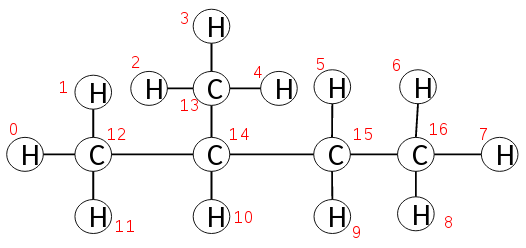
\includegraphics[height=4cm,width=9cm]{images/graphs/C5H12.png}
  \caption{Target Graph}
  \label{C5H12}
\end{minipage}%
\begin{minipage}[t]{.5\textwidth}
  \centering
  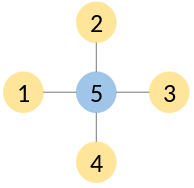
\includegraphics[height=3cm,width=3.3cm]{images/graphs/CH4.png}
  \caption{Pattern graph}
  \label{CH4}
\end{minipage}
\end{figure}
%%%%%%%%%%%%%%%%%%%%%%%%%%%%%%%%%%%%%%%%%%%%%%%%%%%%%%%%%%%%%%%%%%%%%%%%%%%
After candidate extraction, $Path$-$index$ returns target graph \ref{C5H12} as candidate for subgraph isomorphism with pattern graph \ref{CH4}, as all paths in \ref{CH4}, shown on figure \ref{CH4-paths} are contained in \ref{C5H12}, as it can be seen on figure \ref{C5H12-paths}.\par
%When the set of targets is the same for multiple patterns, the target index is still computed only once and reused. The 
%%%%%%%%%%%%%%%%%%%%%%%%%%%%%%%%%%%%%%%%%%%%%%%%%%%%%%%%%%%%%%%%%%%%%%%%%%%
\begin{figure}[H]
\centering
\begin{minipage}[t]{.5\textwidth}
  \centering
  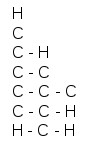
\includegraphics[height=3.3cm,width=2.3cm]{images/paths/C5H12.png}
  \caption{Target graph path enumeration}
  \label{C5H12-paths}
\end{minipage}%
\begin{minipage}[t]{.5\textwidth}
  \centering
  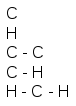
\includegraphics[height=2.4cm,width=2cm]{images/paths/CH4.png}
  \caption{Pattern graph path enumeration}
  \label{CH4-paths}
\end{minipage}
\caption{All paths up to maximum length 3}
\label{pathsEnumeration}
\end{figure}
%%%%%%%%%%%%%%%%%%%%%%%%%%%%%%%%%%%%%%%%%%%%%%%%%%%%%%%%%%%%%%%%%%%%%%%%%%%
\subsection{Implementation}
\label{path-index:implementation}
\subsubsection{Graph representation}
\label{path-index:graph-representation}
	Each graph is represented with a Java class \textrm{Graph} that has an integer id and a collection of node objects as fields, where the integer is a unique identifier. Each node object has an id, a label and a list of edge objects, where the node is a source node for each edge contained in the list. The length of the list of the edge object is equal to the degree of the node. Therefore, each edge object does not need to keep a record of the source node: it only has a label and a destination node as fields. As the graphs we are working with are not directed, two Edge objects are created to represent an edge. The first object has one of the nodes as destination node and then added in the list of edges of the other node: the source node. The second edge object will have the source node of the first edge object as destination node and included in the list of edges of the destination node of the first edge object, which will be its source node. The label of both edge objects will be the same.\par
%%%%%%%%%%%%%%%%%%%%%%%%%%%%%%%%%%%%%%%%%%%%%%%%%%%%%%%%%%%%%%%%%%%%%%%%%%%
\subsubsection{Path Extraction}
\label{path-index:path-extraction}
A class, called \textrm{PathExtractor}, contains all functionality for computing the paths and path-strings that are stored in the index. To compute the index of a given graph dataset, we use the functionality of \textrm{PathExtractor} to extract all paths of every graph in the dataset. The path extraction algorithm is recursive depth-first-search based and is called on every node of the graph. Algorithm 1 describes our approach. Before we call function \textrm{generatePath}, we initialize an empty stack that is used in the algorithm to store visited nodes. \textrm{Algorithm 1} generates all paths in the graph of size $maxL$ , where $maxL$ is the number of nodes in a path, using two functions: \textrm{generatePath} and \textrm{generatePathInner}. The function \textrm{generatePath} in \textrm{Algorithm 1} takes a list of all nodes in the graph and path length $maxL$ as parameters and calls \textrm{generatePathInner} for every node in the list as starting node (line 4). The start node is also pushed on the stack (line 3), as it is part of the path that is to be generated. \par
%%%%%%%%%%%%%%%%%%%%%%%%%%%%%%%%%%%%%%%%%%%%%%%%%%%%%%%%%%%%%%%%%%%%%%%%%%%
\begin{table}[h]
 \centering
 \label{Algorithm 1.}
 \begin{tabular}{l l}
	\textbf{Algorithm 1.} Paths extraction \\\hline
    \small\textbf{1}  \,\small{generatePath(nodes, maxL) $\rightarrow$ void}\\
    \small\textbf{2}  \,\,\,\,\,\,\,\,\small{\textbf{for every} start-node in nodes \textbf{do}:}\\
    \small\textbf{3}  \,\,\,\,\,\,\,\,\,\,\,\,\,\small{push start-node on top of stack}\\
    \small\textbf{4}  \,\,\,\,\,\,\,\,\,\,\,\,\,\small{generatePathInner(node, maxL)}\\
    \small\textbf{5}  \\
    \small\textbf{6}  \,\small{generatePathInner(node, maxL) $\rightarrow$ void}\\
    \small\textbf{7}  \,\,\,\,\,\,\,\,\small{\textbf{if} stack is \textbf{ less or equal to} maxL \textbf{then:}}\\
    \small\textbf{8}  \,\,\,\,\,\,\,\,\,\,\,\,\,\,\small{outputPath(stack)}\\
    \small\textbf{9}  \,\,\,\,\,\,\,\,\small{\textbf{if} stack is \textbf{equal to} maxL \textbf{then:}}\\
    \small\textbf{10} \,\,\,\,\,\,\,\,\,\,\,\,\,\small{remove the topmost element from the stack}\\
    \small\textbf{11} \,\,\,\,\,\,\,\,\,\,\,\,\small{\textbf{exit}}\\
    \small\textbf{12} \,\,\,\,\,\,\,\small{\textbf{for every} neighbor of node:}\\
    \small\textbf{13} \,\,\,\,\,\,\,\,\,\,\,\,\,\small{\textbf{if} neighbor not on stack \textbf{then:}}\\
    \small\textbf{14} \,\,\,\,\,\,\,\,\,\,\,\,\,\,\,\,\,\,\,\,\,\,\,\,\small{push neighbor on top of stack}\\
    \small\textbf{15} \,\,\,\,\,\,\,\,\,\,\,\,\,\,\,\,\,\,\,\,\,\,\,\,\small{\textbf{generatePathInner}(neighbor, maxL)}\\
    \small\textbf{16} \,\,\,\,\,\,\,\small{\textbf{if} all neighbors are on stack \textbf{and} stack is not empty \textbf{then:}}\\
    \small\textbf{17} \,\,\,\,\,\,\,\,\,\,\,\,\,\small{remove the topmost element from the stack}\\
    \hline
 \end{tabular}%
\end{table}
%%%%%%%%%%%%%%%%%%%%%%%%%%%%%%%%%%%%%%%%%%%%%%%%%%%%%%%%%%%%%%%%%%%%%%%%%%%
%TODO explain lines 7 - 11 and check the correctness of line numbers
The recursive function \textrm{generatePathInner} generates all paths is length $maxL$, where the length of a path is equal to the number of all nodes that are part of it, from a start node $node$. First, the size of the stack is checked. If it is less or equal to $maxL$, the contents of the stack are copied and passed to a function \textrm{putToIndex} that computes the string representation of the extracted path and puts it to the index. If the stack is equal to $maxL$, the last element from the stack is popped out and the function exits. If the size of the stack is less than $maxL$, we traverse the neighborhood of $node$ in the for loop, starting at line 12. Every unvisited neighbor of $node$ is pushed on the stack and then a recursive call to \textrm{generatePathInner} is made with the same neighbor node as $node$(lines 13 and 14).\par
%%%%%%%%%%%%%%%%%%%%%%%%%%%%%%%%%%%%%%%%%%%%%%%%%%%%%%%%%%%%%%%%%%%%%%%%%%%
The stack used in \textrm{Algorithm 1} follows the principles of the stack datastructure. In this work, we use the Java implementation. The stack has two main functions: to keep track of the visited nodes in the current function call so that no node takes part in a path more than twice, i.e. there are no cycles; and it contains nodes that always form a valid path. The reason why this is the case is that every time a node is pushed on top of the stack, this node is one of the neighbors of the last node on the stack. The only place in generatePathInner function where new node is added in the stack is in line 14 and the node that is pushed on top of the stack belongs to the list of neighbors of $node$, which is always the previous node in the stack. Therefore, the sequence of all nodes on the stack forms a valid path, as every node is connected with an edge with its predecessor and successor in the sequence. The complexity of Algorithm 1 is explained in section \ref{path-index:complexity}.\par
%%%%%%%%%%%%%%%%%%%%%%%%%%%%%%%%%%%%%%%%%%%%%%%%%%%%%%%%%%%%%%%%%%%%%%%%%%%
The function \textrm{outputPath} is called by \textrm{generatePathInner} every time the stack reaches a size equal to $maxL$ (line 8, Algorithm 1). Algorithm 2 derives the lexicographically smallest string representation of a path, following the principles described in section \ref{path-index-idea}. The resulting path-string is added to the index, if it does not exist there (line 8, Algorithm 2). \par 
Algorithm 2 takes a sequence of nodes as a parameter, which are the contents of the stack when the stack size is $maxL$ (line 8, Algorithm 1). We derive the path-string of the sequence (line 2) that consists of the node label of every node in nodeSequence and the label of the edge it has with the previous node in the path. If the dataset does not have edge labels, a default character is used as label for every edge. In the previous examples, we use the character $"-"$ (figures \ref{C5H12-paths} and \ref{CH4-paths}). It is important to note that the node labels are ordered in exactly the same way as the nodes in the sequence, for example if a node A is on place \textit{i} in the sequence, the label of A will be at place \textit{i} in the string if the edge labels in the string are not counted (if they are counted, the label of A is at position \textit{i} x \textit{2}).\par
Next steps are to compute the reversed sequence of the path (line 3), its string representation (line 4) and check whether the reversed string is lexicographically smaller then the path-string (line 5). If yes, we assign the path-string to be equal to the reversed string (line 6) and add it to the index, if it is not present there yet (line 8). We do not sort the path-string lexicographically, due to the reasons explained in section \ref{path-index-idea}. The complexity of Algorithm 2 is explained in section \ref{path-index:complexity}.\par
%%%%%%%%%%%%%%%%%%%%%%%%%%%%%%%%%%%%%%%%%%%%%%%%%%%%%%%%%%%%%%%%%%%%%%%%%%%
% output path
\begin{table}[h]
 \centering
 \label{Algorithm 2.}
 \begin{tabular}{l l}
	\textbf{Algorithm 2.} Output path \\\hline
    \small\textbf{1} \,\,\small{outputPath(nodeSequence) $\rightarrow$ void}\\
     \small\textbf{2} \,\,\,\,\,\,\,\,\small{pathStr = nodeSequence.toString()}\\
    \small\textbf{3} \,\,\,\,\,\,\,\,\small{reversedSequence = nodeSequence.reverse()}\\
     \small\textbf{4} \,\,\,\,\,\,\,\,\small{pathStrReversed = reversedSequence.toString()}\\
    \small\textbf{5} \,\,\,\,\,\,\,\,\small{\textbf{if} pathStrReversed $<$ pathStr \textbf{then:}}\\
    \small\textbf{6} \,\,\,\,\,\,\,\,\,\,\,\,\,\,\small{pathStr = pathStrReversed}\\
    \small\textbf{7} \,\,\,\,\,\,\,\,\small{\textbf{if} pathStr \textbf{not in} index \textbf{then:}}\\
    \small\textbf{8} \,\,\,\,\,\,\,\,\,\,\,\,\,\,\small{put pathStr to index}\\
    \small\textbf{9}\,\,\,\,\,\,\,\,\small{\textbf{exit}}\\\hline
 \end{tabular}
\end{table}
%%%%%%%%%%%%%%%%%%%%%%%%%%%%%%%%%%%%%%%%%%%%%%%%%%%%%%%%%%%%%%%%%%%%%%%%%%%
%TODO the bug I had initially, how the stack was fixed
% TODO reference Java stack below
% TODO explain about the current maximum path length
% TODO explain isVisited boolean field in the Node class
%Iteration is every new entering to the while loop when we have new start node and we have the stack cleaned up. --- write that properly
%%%%%%%%%%%%%%%%%%%%%%%%%%%%%%%%%%%%%%%%%%%%%%%%%%%%%%%%%%%%%%%%%%%%%%%%%%%
\subsubsection{Candidates extraction}
\label{path-index:candidates-extraction}
Candidates extraction is the part of the implementation where the set of candidates $C$ from the dataset with target graphs is constructed. Algorithm 3 describes our approach in more detail. Function \textrm{candidatesExtractor} takes the index of one graph from the target dataset and the index of the pattern (or one of the set of pattern graphs, if there are more than one pattern) as parameters (line 1). For every path-string in the pattern, we check whether it is contained in the target index (line 3). If yes, the algorithm continues, because the target might be a candidate (line 6). Otherwise, if the pattern path-string does not exist in the target index, the program returns false and terminates (line 4). The program goes to line 7 iff all path-strings in the pattern are contained in the target index.\par
The complexity of Algorithm 3 is explained in section \ref{path-index:complexity}. 
%%%%%%%%%%%%%%%%%%%%%%%%%%%%%%%%%%%%%%%%%%%%%%%%%%%%%%%%%%%%%%%%%%%%%%%%%%%
\begin{table}[H]
 \centering
 \label{Algorithm 3.}
 \begin{tabular}{l l}
 \textbf{Algorithm 3.} Candidates extraction \\\hline
 \small\textbf{1} \small{candidatesExtractor(target-index, pattern-index) $\rightarrow$ \textbf{true} or \textbf{false}}\\
 \small\textbf{2} \,\,\,\,\small{\textbf{for every} pattern-path \textbf{in} pattern-index:}\\
 \small\textbf{3} \,\,\,\,\,\,\,\,\small{\textbf{if no} target-path \textbf{equals} pattern-path \textbf{then:}}\\
 \small\textbf{4} \,\,\,\,\,\,\,\,\,\,\,\,\small{\textbf{return false}}\\
 \small\textbf{5} \,\,\,\,\,\,\,\,\small{\textbf{else:}}\\
 \small\textbf{6} \,\,\,\,\,\,\,\,\,\,\,\,\small{\textbf{continue}}\\
 \small\textbf{7} \,\,\,\,\small{\textbf{return true}}\\
 \hline
 \end{tabular}
\end{table}
%%%%%%%%%%%%%%%%%%%%%%%%%%%%%%%%%%%%%%%%%%%%%%%%%%%%%%%%%%%%%%%%%%%%%%%%%%%
\subsection{Performance}
This section gives more details about the complexity of each of the algorithms in the implementation, explained in sections \ref{path-index:path-extraction} and \ref{path-index:candidates-extraction}, continued with statistics about the algorithm running time and performance after running it on various datasets. Following the results obtained, we make a conclusion about the observed performance of the algorithm and analyze its advantages and disadvantages.\par
%%%%%%%%%%%%%%%%%%%%%%%%%%%%%%%%%%%%%%%%%%%%%%%%%%%%%%%%%%%%%%%%%%%%%%%%%%%
\subsubsection{Complexity}
\label{path-index:complexity}
Algorithm 1 works like depth-first search, but the depth of the search has a maximum limit $maxL$. For each target graph, we conduct depth-first search of depth $maxL$. During the search, each neighbor of $maxL$ number of nodes is visited. The worst case complexity is when the target graph is a clique. If we assume that the number of nodes in the clique is n (equal to the number of edges), then the for loop on line 2 will be executed n times, each time calling \textrm{generatePathInner} function. This function will make recursive call for every unvisited neighbor of the current vertex, until the stack reaches size equal to $maxL$. As after every recursive call, the size of the stack is increased by 1 and the graph is a clique, the number of neighbors that will be visited during the next recursive call decreases by 1. The depth of the recursive calls is at most $maxL$ (the maximum size of the path we want  is $maxL$), therefore the function has worst case complexity \textbf{O((n - 1).(n - 2) ... (n - maxL - 1))}, which occurs when the graph is a clique. \par
%%%%%%%%%%%%%%%%%%%%%%%%%%%%%%%%%%%%%%%%%%%%%%%%%%%%%%%%%%%%%%%%%%%%%%%%%%%
 Algorithm 2 does not have any loops, but it calls the function \textrm{toString()}, which traverses the given path once to change each node with its label and an edge label to the next node in the sequence. The \textrm{toString()} method visits every node in the path, takes the label of the current node, and if the dataset has edge labels, finds the edge label of the edge between the current node and the next node, otherwise adds a default character after the node label. On line 7, there is a traversal through the current index of a graph. The complexity of Algorithm 2 is therefore \textbf{O(maxL + index size)}, where index size is the current size of the index for the current graph being indexed. The best case is when the index is empty: then traversing the index takes constant time and the complexity of the \textrm{toString()} method is \textbf{O(maxL)}.\par
%%%%%%%%%%%%%%%%%%%%%%%%%%%%%%%%%%%%%%%%%%%%%%%%%%%%%%%%%%%%%%%%%%%%%%%%%%%
Algorithm 3 visits every path stored in the pattern index and for each pattern path, it goes through the target index and checks whether it contains the same path. This procedure is done for every target graph in the dataset. If we assume that the number of paths in the pattern index is \textit{p}, the number of paths in the current target index is \textit{t} and the number of graphs in the target dataset is \textit{n}, the number complexity of the algorithm is \textbf{O(ptn)}.\par
%%%%%%%%%%%%%%%%%%%%%%%%%%%%%%%%%%%%%%%%%%%%%%%%%%%%%%%%%%%%%%%%%%%%%%%%%%%
\subsection{Experimental Results}
\label{path-index:experimental-results}
TODO


%%%%%%%%%%%%%%%%%%%%%%%%%%%%%%%%%%%%%%%%%%%%%%%%%%%%%%%%%%%%%%%%%%%%%%%%%%%
\subsection{Advantages and Limitations}
\label{path-index:advantages-limitations}
    TODO\\
    - structural information is lost, because path is too simple\\
	- it is computationally intense, i.e. very slow especially when computing paths of higher length; there are too many paths\\
    - very easy to implement\\
    - paths are easier to manipulate than trees and graphs --- why?\\
    - this indexing technique is good when we have graphs with large number of different labels on their nodes and low density of edges between the graphs' nodes\\
    - the index space is predefined: all the paths up to \texttt{maxLen} length are selected\\
%%%%%%%%%%%%%%%%%%%%%%%%%%%%%%%%%%%%%%%%%%%%%%%%%%%%%%%%%%%%%%%%%%%%%%%%%%%
%%%%---------------------- Path-Subtree Index -------------------------%%%%
%%%%%%%%%%%%%%%%%%%%%%%%%%%%%%%%%%%%%%%%%%%%%%%%%%%%%%%%%%%%%%%%%%%%%%%%%%%
\section{Path-Subtree Index}
\label{path-subtree-index}
  $Path$-$Subtree$ index is the second indexing technique that was designed, implemented and evaluated. In this section we explain its main idea, implementation and performance, observed after testing with various types of graph data sets. We write about the problems with the algorithm we discovered after the initial implementation and how we changed $Path$-$Subtree$ index to solve the issues encountered. Lastly, we draw conclusions about the advantages and limitations of this indexing technique.  
\subsection{Initial idea}
%%%%%%%%%%%%%%%%%%%%%%%%%%%%%%%%%%%%%%%%%%%%%%%%%%%%%%%%%%%%%%%%%%%%%%%%%%%%
As mentioned in section \ref{path-index:advantages-limitations}, $Path$ index can't extract most of the structural information present in the graphs. It is almost of no use for targets that have small number of different labels, like the AIDS data set for example. $Path$-$Subtree$ index addresses the problem of insufficient structural information extraction by introducing a novel representation of the paths that takes into account the neighborhood of each node. A new version of the label of each node that is present in the path is computed and stored in the index instead of the node$'$s original label. In this work, we refer to this alternate label as \textit{neighborhood label}. The next paragraphs introduce necessary naming conventions and then describe what \textit{neighborhood label} means and why we believe it helps to derive a better index.\par %%%%%%%%%%%%%%%%%%%%%%%%%%%%%%%%%%%%%%%%%%%%%%%%%%%%%%%%%%%%%%%%%%%%%%%%%%%%
Let \texttt{n} be a node with neighbors \texttt{N} = $\{$ $n^{}_1$, $n^{}_2$ \ldots $n^{}_i$ $\}$, where \texttt{i} is the size of \texttt{N}. Let us define a labeling function \textit{l} that maps the node \texttt{n} and each node in \texttt{N} to a character, also called the node label. We refer to the label of \texttt{n} as \texttt{$L^{}_n$} and the label of each node $n^{}_j$ in \texttt{N}, where $j$ is between $1$ and $i$ inclusive, as \texttt{$L^{}_j$}. It is important to note that using this notation we do not mean that each node has unique label, i.e. there may exist nodes $n^{}_g$ and $n^{}_h$, where $g$ and $h$ are between $1$ and $i$ inclusive, and \texttt{$L^{}_g$} is the same as \texttt{$L^{}_h$}.\par %%%%%%%%%%%%%%%%%%%%%%%%%%%%%%%%%%%%%%%%%%%%%%%%%%%%%%%%%%%%%%%%%%%%%%%%%%%%
The term \texttt{neighborhood label} is a specific label that is computed for each node in the graph using the label of each node and its neighbors: all nodes, connected with an edge with it. The label derived is then stored in the index file as part of the string representation of the nodes in the paths, similarly to the node labels that are part of the string representations of paths in the previous index algorithm in section \ref{path-index}.\par
The \textit{neighborhood label} of \texttt{n} is derived in the following way. Let the label of \texttt{n} and the labels of all members of \texttt{N} form the set of labels \texttt{S}. The \textit{neighborhood label} of \texttt{n} is constructed using the labels in \texttt{S}, ordered lexicographically from the smallest to the largest label in \texttt{S}. For instance, we take each member of \texttt{S} and derive the sequence \texttt{S$'$} = $s^{}_1$$s^{}_2$$s^{}_3$ \ldots $s^{}_i$, where $i$ is the number of the neighbors of \texttt{n} and consequently the number of members of the set of labels \texttt{S}. \texttt{S$'$} is the resulting \textit{neighborhood label} of \texttt{n}. For example, the \textit{neighborhood label} of each node of the graph on figure \ref{CH4} is shown on figure \ref{CH4-subtree-label-graph}, where the red number on the left side of each node is its id. From figure \ref{CH4} it can be seen that node with id 4 has neighbors nodes 0, 1, 2, 3 each of them with label \texttt{H}. The label of node 4 is \texttt{C} and after appending the labels of its neighborhood, the resulting \textit{neighborhood label} is \texttt{CHHHH}. Similarly, the label of node 4 is part of the \textit{neighborhood label} of the other nodes.\par
%%%%%%%%%%%%%%%%%%%%%%%%%%%%%%%%%%%%%%%%%%%%%%%%%%%%%%%%%%%%%%%%%%%%%%%%%%%%
\begin{figure}[h]
  \begin{minipage}[t]{.5\textwidth}
  \centering
  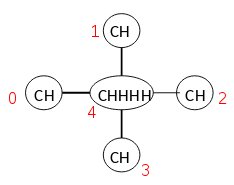
\includegraphics[height=3.8cm,width=4.2cm]{images/graphs/CH4-isomer.png}
  \caption{Subtree-label graph of \ref{CH4}}
  \label{CH4-subtree-label-graph}
  \end{minipage}%
  \begin{minipage}[t]{.5\textwidth}
  \centering
  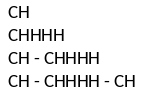
\includegraphics[height=2.2cm,width=2.9cm]{images/paths/CH4-isomer.png}
  \caption{Paths derived from neighborhood labels}
  \label{CH4-subtree-label-paths}
  \end{minipage}
\end{figure}
%%%%%%%%%%%%%%%%%%%%%%%%%%%%%%%%%%%%%%%%%%%%%%%%%%%%%%%%%%%%%%%%%%%%%%%%%%%%
The resulting path-strings from path extraction of \ref{CH4-subtree-label-graph} for $maxL$ equal to 3 are shown on figure \ref{CH4-subtree-label-paths}, where the the character $"-"$ denotes an edge. It is important to note that although the path representation stored in the index file is changed, the original node labels of the graph are not removed so that the structure and labeling remains unchanged. Also, the paths on figure \ref{CH4-subtree-label-paths} are composed from the same nodes as the paths of figure \ref{CH4-paths}. The difference of the representation comes only from the alternative labeling model. The method of extracting the paths remains the same as the one used for $Path$ index and described in section \ref{path-index}. Similarly, computing the set of graphs possibly subgraph isomorphic to a pattern graph \texttt{p}, also called the \textit{candidate set}, is done using the same method as $Path$ index.\par
%%%%%%%%%%%%%%%%%%%%%%%%%%%%%%%%%%%%%%%%%%%%%%%%%%%%%%%%%%%%%%%%%%%%%%%%%%%%
Like $Path$ index, $Path$-$Subtree$ index supports graphs that have labels on edges and nodes. When deriving the representation of each path that is later stored in the index, we include the label of the edge that connects every two nodes \texttt{a} and \texttt{b} that are part of the path. If we take the graph on figure \ref{CH4-subtree-label-graph}, we notice that there are no labels of its edges. Consequently, the paths stored in the target index, also shown on figure \ref{CH4-subtree-label-paths} have the character $"-"$ between the \textit{neighborhood label} of each two nodes. If graph \ref{CH4-subtree-label-graph} had edge labels, we would include the corresponding label instead of $"-"$. \par  
%%%%%%%%%%%%%%%%% WHY IS NEIGHBORHOOD METHOD BETTER? %%%%%%%%%%%%%%%%%%%
Mathematical proof that the second indexing method is better than the first one. \\


- the path extraction is done in the same way only labels are changed


%%%%%%%%%%%%%%%%%%%%%%%%%%%%%%%%%%%%%%%%%%%%%%%%%%%%%%%%%%%%%%%%%%%%%%%%%%%
With the following example we show that $Path$-$Subtree$ index discriminates graphs that $Path$ index can not. Let us consider the graphs on figure \ref{C2H6} and \ref{CH4}. Let \ref{C2H6} be the target graph and \ref{CH4} to be the pattern. Before running the subgraph isomorphism test on the two graphs, we will index them and see whether we can filter out \ref{C2H6}. As we can see, \ref{C2H6} does not contain \ref{CH4} and we are going to check whether Index-2 will return the target graph as a false-positive candidate for subgraph isomorphism with our pattern. After computing the indexes of the two graphs, we get the results for \ref{C2H6} shown on figure \ref{C2H6-subtree-label-paths} and the results for \ref{CH4} on figure \ref{CH4-subtree-label-paths}. As we can see from the figures, the index of our pattern graph has paths that the target does not contain, for example \texttt{CHHHH, CH-CHHHH, CH-CHHHH-CH}. The target graph is not returned as a candidate for subgraph isomorphism. Computing the index using $Path$ index results in getting the paths, displayed on figure \ref{C2H6-paths} for our target graph \ref{C2H6} and the paths on figure \ref{CH4-paths} for the pattern. As all paths of \ref{CH4} are contained in the index of \ref{C2H6}, $Path$ index returns \ref{C2H6} as candidate for subgraph isomorphism.\par
%%%%%%%%%%%%%%%%%%%%%%%%%%%%%%%%%%%%%%%%%%%%%%%%%%%%%%%%%%%%%%%%%%%%%%%%%%%
\begin{figure}[h]
  \begin{minipage}[t]{.3\textwidth}
    \centering
    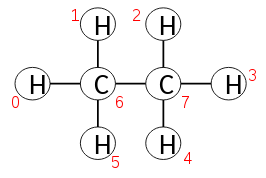
\includegraphics[height=2.6cm,width=3.6cm]{images/graphs/C2H6.png}
    \caption{Target graph}
    \label{C2H6}
  \end{minipage}
  \begin{minipage}[t]{.3\textwidth}
  \centering
  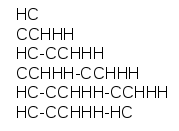
\includegraphics[height=3.3cm,width=4.3cm]{images/paths/C2H6-isomer-paths.png}
  \caption{Subtree-label paths}
  \label{C2H6-subtree-label-paths} %%%this figure is wrong!!! it is not HC, it is CH here
  \end{minipage}
  \begin{minipage}[t]{.3\textwidth}
  \centering
  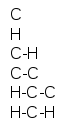
\includegraphics[height=3.3cm,width=1.6cm]{images/paths/C2H6-paths.png}
  \caption{Paths}
  \label{C2H6-paths}
  \end{minipage}
\end{figure}
%%%%%%%%%%%%%%%%%%%%%%%%%%%%%%%%%%%%%%%%%%%%%%%%%%%%%%%%%%%%%%%%%%%%%%%%%%%%
\subsection{Problems with Path-Subtree index}
\label{path-subtree index problems}
After we implemented $Path$-$Subtree$ index based on the principles described in the previous subsection, we discovered that our algorithm is wrong. Apart from the expected false positives, it had false negatives. False negatives in this case are target graphs that contain the pattern, but are wrongly filtered out after the graph indexing step and are never included in the candidate set. The existence of false negatives is strongly undesired, as it is an indication that the indexing algorithm is wrong and therefore useless. We discovered what the reason for discarding targets wrongly is. In the following paragraphs we explain in more details the problem using a worked example and propose a modification of the algorithm that has the potential to solve the issue.\par
%%%%%%%%%%%%%%%%%%%%%%%%%%%%%%%%%%%%%%%%%%%%%%%%%%%%%%%%%%%%%%%%%%%%%%%%%%%%
Let the graph on figure \ref{C2H6} be our target graph and the graph on figure \ref{C2H3} be the pattern. As we can see from the two figures, \ref{C2H6} contains \ref{C2H3} and we expect that a correct indexing technique will return \ref{C2H3} as a candidate for subgraph isomorphism check. After computing the indexes of the target and the pattern graphs, we derive the results for the target, shown on figure \ref{C2H6-subtree-label-paths}, and for the pattern, shown on figure \ref{C2H3-subtree-label-paths}. As we can see from the two figures, although the target contains the pattern, the paths in their indexes are different. As the target index does not contain paths existent in the pattern index, like \texttt{CC, CC-CCHHH} and \texttt{CH-CCHHH-CC} for instance. In this case, \ref{C2H6} is a false negative, discarded wrongly because of our incorrect indexing technique.\par
%%%%%%%%%%%%%%%%%%%%%%%%%%%%%%%%%%%%%%%%%%%%%%%%%%%%%%%%%%%%%%%%%%%%%%%%%%%%
\begin{figure}[h]
  \begin{minipage}[t]{.5\textwidth}
    \centering
    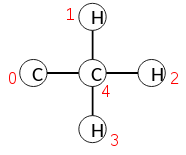
\includegraphics[height=3.3cm,width=3.7cm]{images/graphs/C2H3.png}
    \caption{Pattern graph}
    \label{C2H3}
  \end{minipage}
  \begin{minipage}[t]{.5\textwidth}
  \centering
  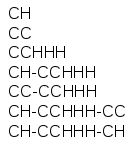
\includegraphics[height=3.9cm,width=3.8cm]{images/paths/C2H3-isomer-paths.png}
  \caption{Subtree-label paths}
  \label{C2H3-subtree-label-paths}
  \end{minipage}
\end{figure}
%%%%%%%%%%%%%%%%%%%%%%%%%%%%%%%%%%%%%%%%%%%%%%%%%%%%%%%%%%%%%%%%%%%%%%%%%%%%
\subsection{Algorithm Refinement}
  In order to solve the problem with false negatives, we changed the candidate extraction part. For every path $pp$ in the pattern index, we check which target graphs contain $pp$ as a path. Let us have $pp$ = \texttt{CH-CCHHH} and we want to check it against the target path $tp$ = \texttt{CH-CCCHHH-CHHH}. For every \textit{neighborhood label} in $pp$, our algorithm will whether it is contained in the corresponding label in $tp$. We first compare \texttt{CH} and \texttt{CH}, and as they are equal, we continue with the labels on the next position: \texttt{CCHHH} and \texttt{CCCHHH}. As \texttt{CCCHHH} contains \texttt{CCHHH} and this is the last label in $pp$, we stop and return true, $tp$ contains $pp$.\par
%%%%%%%%%%%%%%%%%%%%%%%%%%%%%%%%%%%%%%%%%%%%%%%%%%%%%%%%%%%%%%%%%%%%%%%%%%%%
Using the refinement described above, we removed the problem with false negatives, described in section \ref{path-subtree index problems}. However, this results in weaker filtering power. Now, there are some cases where $path$-$index$ would perform better, although it extracts less structural information about the graphs. We will show how our refined method introduces more false-positives using an example. Let us consider the two graphs on figures \ref{C2H4-1} and \ref{C2H}. Let us apply the refined $Path$-$Subtree$ indexing method for the two graphs, where \ref{C2H} is the pattern and \ref{C2H4-1} is the target (clearly, \ref{C2H4-1} does not contain \ref{C2H} as subgraph). The \textit{neighborhood labels} of the target and the pattern for $maxL$=3 are shown on figures \ref{C2H4-1-subtree-label-paths} and \ref{C2H-subtree-label-paths} respectively. Applying the new candidate extraction technique, we will have \ref{C2H4-1} returned as candidate, because it contains all paths in \ref{C2H}.\par
%%%%%%%%%%%%%%%%%%%%%%%%%%%%%%%%%%%%%%%%%%%%%%%%%%%%%%%%%%%%%%%%%%%%%%%%%%%%  
\begin{figure}[h]
\centering
\begin{minipage}[t]{.5\textwidth}
  \centering
  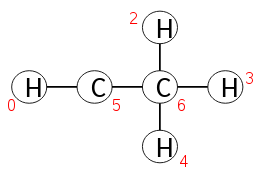
\includegraphics[height=3cm,width=4.5cm]{images/graphs/C2H4-1.png}
  \caption{Graph A}
  \label{C2H4-1}
\end{minipage}%
\begin{minipage}[t]{.5\textwidth}
  \centering
  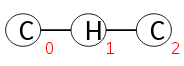
\includegraphics[height=1.2cm,width=3cm]{images/graphs/C2H.png}
  \caption{Graph B}
  \label{C2H}
\end{minipage}%

\begin{minipage}[t]{.5\textwidth}
  \centering
  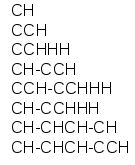
\includegraphics[height=4.4cm,width=3.9cm]{images/paths/C2H4-1-isomer-paths.png}
  \caption{Neighborhood label paths of A}
  \label{C2H4-1-subtree-label-paths}
\end{minipage}%
\begin{minipage}[t]{.5\textwidth}
  \centering
  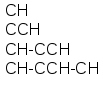
\includegraphics[height=2.1cm,width=2.7cm]{images/paths/C2H-isomer-paths.png}
  \caption{Neighborhood label paths of A}
  \label{C2H-subtree-label-paths}
\end{minipage}%
\end{figure}
%%%%%%%%%%%%%%%%%%%%%%%%%%%%%%%%%%%%%%%%%%%%%%%%%%%%%%%%%%%%%%%%%%%%%%%%%%%%
Let us examine in more detail the only path of length 3 in the pattern graph. It is composed from the nodes with ids \texttt{0, 1} and \texttt{2}. Using $Path$-$Subtree$ index method, this path is represented as \texttt{CH-CCH-CH} in the index file. If we used $path$-$index$, we would store this path as the string \texttt{C-H-C}. Although the path representation \textit{neighborhood label} gives us more information about the node neighbors, with us we loose important structural information, which is: the label of the actual node. In the string \texttt{CCH},  either of the letters could be the label of the node. As shown in the example above, this confusion leads to more false positives.\par
%%%%%%%%%%%%%%%%%%%%%%%%%%%%%%%%%%%%%%%%%%%%%%%%%%%%%%%%%%%%%%%%%%%%%%%%%%%%
TODO
  - we changed the string representation of the isomer label. First letter is always the original label, the others are from the neighbors, sorted in lexicographic order\\
 %%%%%%%%%%%%%%%%%%%%%%%%%%%%%%%%%%%%%%%%%%%%%%%%%%%%%%%%%%%%%%%%%%%%%%%%%%% 
\begin{figure}[h]
\centering
\begin{minipage}[t]{.5\textwidth}
  \centering
  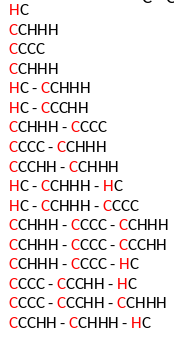
\includegraphics[height=8cm,width=4cm]{images/paths/C5H12-isomer.png}
  \caption{Target graph path enumeration}
  \label{C5H12-isomer-paths}
\end{minipage}%
\begin{minipage}[t]{.5\textwidth}
  \centering
  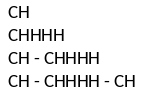
\includegraphics[height=2.3cm,width=3.3cm]{images/paths/CH4-isomer.png}
  \caption{Pattern graph path enumeration}
  \label{CH3-isomer-paths}
\end{minipage}
\caption{All paths up to maximum length 3}
\label{isomer-paths-enumeration}
\end{figure}
%%%%%%%%%%%%%%%%%%%%%%%%%%%%%%%%%%%%%%%%%%%%%%%%%%%%%%%%%%%%%%%%%%%%%%%%%%%%
\subsection{Implementation}
       
       - extend IB-Index 1 and put an option to extract paths using isomer labels.\\
       - describe the extension of the project to support both types of indexing.\\
       - when parsing the graphs, after parsing each graph, compute the isomer label of every node for this graph\\
       - additional field in Node class for isomer labels\\
       - we have a class Path to represent the paths. Each path is an array of nodes. There is a toString method that returns the desired string that we are to store in the index. Depending on the option, we can return path from the labels (ib-index 1), path from the isomer labels (ib-index 2) or a path from the id of each node, made for testing purposes There is a method to reverse the path and it is used when storing the paths in the index: we always store the lexicographically smaller path, comparing each path with its reversed equivalent.\\
       - re-written the candidates extraction part. We have to check for containment ... \\
%%%%%%%%%%%%%%%%%%%%%%%%%%%%%%%%%%%%%%%%%%%%%%%%%%%%%%%%%%%%%%%%%%%%%%%%%%%%  
\subsection{Performance}
TODO \\
       - the index file is bigger, but the candidate set is smaller\\
       - put the table with results\\
       - explain the results and why they are like this\\
	   - complexity?\\
 	   - what could be done better and how?\\
%%%%%%%%%%%%%%%%%%%%%%%%%%%%%%%%%%%%%%%%%%%%%%%%%%%%%%%%%%%%%%%%%%%%%%%%%%%%
\subsection{Variants of Path-Subtree index}
TODO \\
 %- use neighborhood of length 2, 3 ...
 %- this will result in bigger index, but even stronger filtering strength, which means
%%%%%%%%%%%%%%%%%%%%%%%%%%%%%%%%%%%%%%%%%%%%%%%%%%%%%%%%%%%%%%%%%%%%%%%%%%%%
\subsection{Advantages and Limitations}
TODO \\
 - very easy to implement, especially when we have index-1 implementation ready\\
 %- the index file is even bigger --- this is  bad\\
%%%%%%%%%%%%%%%%%%%%%%%%%%%%%%%%%%%%%%%%%%%%%%%%%%%%%%%%%%%%%%%%%%%%%%%%%%%%
%%%------------------------------IB-Index 3------------------------------%%%
%%%%%%%%%%%%%%%%%%%%%%%%%%%%%%%%%%%%%%%%%%%%%%%%%%%%%%%%%%%%%%%%%%%%%%%%%%%%
\section{IB-Index 3}
TODO and to implement
isomers + different graph representation (array, bitset, hashing)
maximal paths
        
\section{Test harness}
TODO \\
- junit tests for each method ...\\
- what tests we did and why\\


\chapter{Experimental Evaluation}
    \section{Experimental Data and Methodology}
    \section{Results Summary}
    
\chapter{Conclusion and Future work}

%%%%%%%%%%%%%%%%
%              %
%  APPENDICES  %
%              %
%%%%%%%%%%%%%%%%
\begin{appendices}

\chapter{Running the Programs}
An example of running from the command line is as follows:
\begin{verbatim}
      > java MaxClique BBMC1 brock200_1.clq 14400
\end{verbatim}
This will apply $BBMC$ with $style = 1$ to the first brock200 DIMACS instance allowing 14400 seconds of cpu time.

\chapter{Generating Random Graphs}
\label{sec:randomGraph}
We generate Erd\'{o}s-R\"{e}nyi random graphs $G(n,p)$ where $n$ is the number of vertices and
each edge is included in the graph with probability $p$ independent from every other edge. It produces
a random graph in DIMACS format with vertices numbered 1 to $n$ inclusive. It can be run from the command line as follows to produce 
a clq file
\begin{verbatim}
      > java RandomGraph 100 0.9 > 100-90-00.clq
\end{verbatim}
\end{appendices}

%%%%%%%%%%%%%%%%%%%%
%   BIBLIOGRAPHY   %
%%%%%%%%%%%%%%%%%%%%

\bibliographystyle{plain}
\bibliography{bib}

\end{document}
